%!TEX root =  main.tex
\section{Introduction}

State machine replication (SMR) is a fundamental technique for
building fault tolerant systems and services. With SMR, state is
replicated on a set of servers, and each replica deterministically
executes the same sequence of client commands in order to maintain
consistency. Unfortunately, increasing the number of replicas can
negatively impact performance, since each replica must execute every
command.  In order to improve the scalability of SMR, several systems
have investigated the use of state partitioning~\cite{facebookTAO,
  sciascia2012sdur, Aguilera:2007}.

In principle, increasing the number of partitions should result in
increased system performance. However, if executing an operation
requires that the system access multiple partitions, then performance
can actually decrease, due to overhead from ordering commands to
ensure strong consistency. On the other hand, placing data in a single
partition can result in load imbalances, nullifying the benefits of
partitioning.  Thus, an ideal partitioning scheme is one that would
both (i) minimize multiple partition commands, and (ii) provide load
balancing among the partitions. We refer to workloads that can be
partitioned in a way that satisfies these two properties as exhibiting
\emph{strong locality}.

Broadly speaking, there are two classes of techniques for
partitioning. \emph{Static} schemes choose an optimal partitioning
based on the workload, and never change the assignment of objects to
partitions. Such approaches require a priori knowledge of the
workload~\cite{curino2010sch} and cannot adapt as workloads change
over time (e.g., in social networks users join and leave the system,
connections are created and removed).  \emph{Dynamic} techniques move
data to partitions in order to avoid multi-partition
commands~\cite{long16}. Unfortunately, existing dynamic schemes assume
workloads with strong locality, or suffer from instability due to
constantly moving data from one partition to another.


In this paper, we introduce \dynastar, a new approach to the state
partitioning problem designed to address these challenges.  \dynastar
is \emph{dynamic}. It does not require any a priori knowledge about
the workload, and it adapts to workload changes on-the-fly. However,
in contrast to existing dynamic schemes, \dynastar minimizes the
number of state relocations by monitoring the workload, and
periodically re-computing an optimal partitioning using the static
METIS partitioning algorithm~\cite{Abou-Rjeili:2006}.


With \dynastar, a location oracle maintains two data structures: (i) a
mapping of objects to partitions, and (ii) a \emph{workload graph}
with objects as vertices and edges as commands that access the
objects.  When a client submits a command, it must first contact the
location oracle to discover the partitions on which the objects are
stored.  If the command accesses objects in multiple partitions, the
oracle issues a move command to the partitions, re-locating objects to
a single partition. Of course, when re-locating an object, the oracle
is faced with a choice of which partition to use as a destination.
\dynastar chooses the optimal partition for relocation (i.e., one that
would minimize the number of state relocations) by periodically
partitioning of the workload graph using the METIS.



\noindent
\textbf{Motivating example.}
As both a motivating example, and a preview of the benefits of
\dynastar, we experimentally evaluate the decentralized scheme
proposed by Long et al.~\cite{hoang2016} with workloads that exhibit
strong and weak locality.  We also compare the technique to an
optimized static partitioning scheme, hereafter, referred to as
\emph{optimized partitioning}.  The optimized partitioning scheme uses
METIS~\cite{Abou-Rjeili:2006} to compute a partitioning of the
workload graph and then distribute variables among partitions before the
system starts.  METIS creates balanced partitions with a near-minimum
number of edges across partitions.  In the decentralized partitioning
scheme, variables are randomly distributed among partitions at startup
and then moved across partitions as the execution evolves.  With
strong locality, METIS decomposes the workload graph into connected
components, one per partition.  With weak locality, METIS partitions
the workload so that approximately 1\% of edges connect variables in
different partitions.  Notice that the optimized scheme is intended as
a reference for performance, as it requires complete a priori
knowledge about the workload.

Figure~\ref{fig:motivation} shows the results.  With strong locality,
the decentralized scheme experiences a large number of move operations
until each connected component is entirely contained in a partition
(left top graph).  Once this happens, throughput of the scheme is
similar to the throughput of the optimized scheme (left bottom graph).
With weak locality, though, move operations happen throughout the
whole execution (right top graph).  In this case, throughput is
substantially lower than what the optimized scheme can achieve (right
bottom graph).



\begin{figure*}[ht]
	\center
	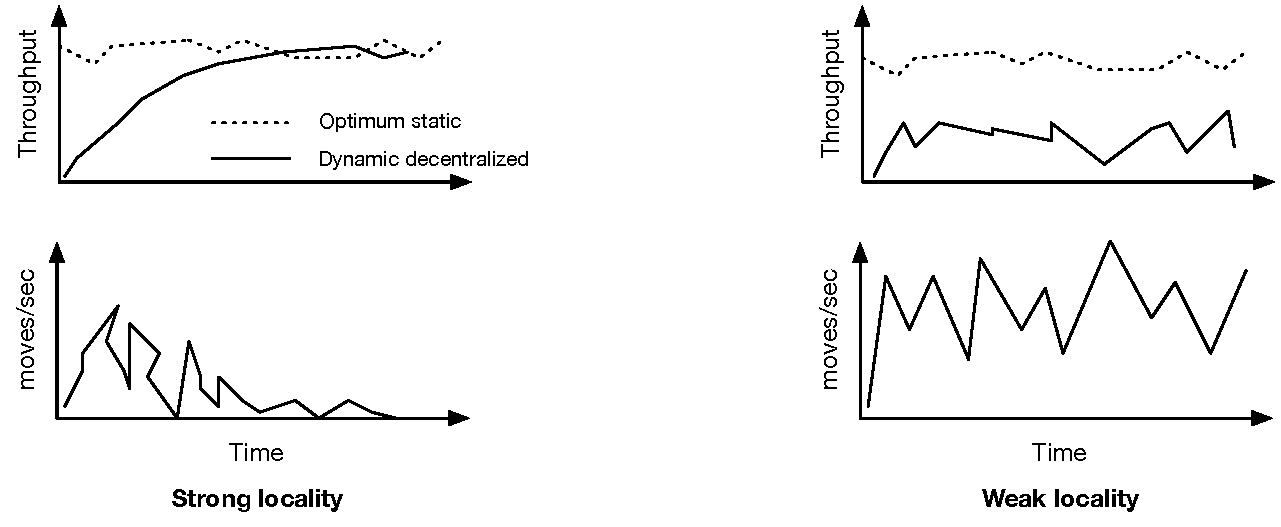
\includegraphics[width=0.6\linewidth]{figures/motivation}
	\caption{Performance under strong and weak locality.}
	\label{fig:motivation}
\end{figure*}



\smallskip


We have fully implemented \dynastar and compared its performance to
the dynamic partitioning protocol proposed by Long et
al.~\cite{hoang2016} and to the optimized static partitioning scheme.
Our prototype can handle workload graphs with half a million variables
and tens of millions of connections.  In workloads that present strong
locality, all three protocols eventually delivered comparable
performance, although \dynastar converged more quickly than the
decentralized scheme.  In workloads with weak locality, however,
\dynastar \emph{outperformed both} schemes.  The reason for the
surprisingly high performance of \dynastar compared to the optimized
static partitioning scheme is that \textbf{we need to explain this!!!
  :-)}

The paper makes the following contributions:
\begin{itemize}
\item It introduces \dynastar and discusses its implementation. 
\item It evaluates different partitioning schemes for state machine replication under a variety of conditions.
\item It describes \appname{} to demonstrate how \libname{} can be used to implement a scalable social network service.
\item It presents a detailed experimental evaluation of \dynastar including real social network graphs with half a million users and 14 million edges.
\end{itemize}

The rest of the paper is structured as follows.
Section~\ref{sec:sysmodel} describes our system model.
Section~\ref{sec:background} reviews existing scalable state machine replication approaches.
Section~\ref{sec:dssmr} introduces \dssmr{}; we explain the technique in detail and argue about its correctness.
Section~\ref{sec:implementation} details the implementation of \libname\ and \appname{}.
Section~\ref{sec:experiments} reports on the results of our experiments with \dssmr{}.
Section~\ref{sec:rw} surveys related work and
Section~\ref{sec:conclusion} concludes the paper.



%The main contribution of this paper is a dynamic partitioning scheme that \emph{performs comparably to the optimum static scheme but with no a priori knowledge about the workload}.


%%State machine replication (SMR) is a well-established technique to develop highly available services (e.g., \cite{Shvachko:2003,Ghemawat:2003,Burrows:2006,MacCormick:2004}).
%%In essence, the idea is that replicas deterministically execute the same sequence of client commands in the same order and in doing so traverse the same sequence of states and produce the same results.
%%State machine replication provides configurable fault tolerance in the sense that the system can be set to tolerate any number of faulty replicas.
%%%Increasing the number of replicas, however, will not scale performance since each replica must execute every command.
%%Unfortunately, increasing the number of replicas will not scale performance since each replica must execute every command.
%%
%%%For many online services, caping performance is a serious drawback.
%%Conceptually, scalable performance can be achieved with state partitioning (e.g., \cite{facebookTAO, sciascia2012sdur, Aguilera:2007}).
%%Ideally, if the service state can be divided such that commands access one partition only and are equally distributed among partitions, then system throughput (i.e., the number of commands that can be executed per time unit) will increase linearly with the number of partitions.
%%Although promising, exploiting partitioning in SMR is challenging.
%%First, most applications cannot be partitioned in such a way that commands always fall within a single partition.
%%Therefore, a partitioning scheme must cope with multi-partition commands.
%%Second, determining an efficient partitioning of the state is computationally expensive and requires an accurate characterization of the workload.
%%
%%There are two general solutions to handle multi-partition commands.
%%One solution is to weaken the guarantees of commands that involve multiple partitions (e.g., \cite{facebookTAO}).
%%In the context of SMR, this would mean that single-partition commands are strongly consistent (i.e., linearizable) but multi-partition commands are not.
%%Another solution is to provide strong consistency guarantees for both single- and multi-partition commands, at the cost of a more complex execution path for commands that involve multiple partitions.
%%\ssmrlong\ (\ssmr)~\cite{bezerra2014ssmr} is a solution in this category.
%%\ssmr\ partitions the service state and replicates each partition.
%%It relies on an atomic multicast primitive to consistently order commands within and across partitions. 
%%Single-partition commands are multicast to their concerned partition and executed just like in classical SMR.
%%Multi-partition commands are multicast to all involved partitions; to prevent command interleaves that violate strong consistency, \ssmr\ implements execution atomicity.
%%With execution atomicity, partitions coordinate during the execution of multi-partition commands.
%%Unsurprisingly, multi-partition commands are more expensive than single-partition commands, and thus, the performance of \ssmr\ is particularly sensitive to the way the service state is partitioned.
%%
%%Determining a partitioning of the state that avoids load imbalances and favors single-partition commands normally requires a good understanding about the workload. 
%%Even if enough information is available, finding a good partitioning is a complex optimization problem~\cite{curino2010sch,taft2014est}.
%%Moreover, many online applications experience variations in demand. 
%%These happen for a number of reasons. 
%%In social networks, some users may experience a surge increase in their number of followers (e.g., new ``celebrities");
%%workload demand may shift along the hours of the day and the days of the week; and unexpected (e.g., a video that goes viral) or planned events (e.g., a new company starts trading in the stock exchange) may lead to exceptional periods when requests increase significantly higher than in normal periods.
%%\ssmr\ assumes a static workload partitioning.
%%Any state reorganization requires system shutdown and manual intervention.
%%
%%Given these issues, it is crucial that highly available partitioned systems be able to dynamically adapt to the workload.
%%In this paper, we present \dssmrlong\ (\dssmr), a technique that allows a partitioned SMR system to reconfigure its data placement on-the-fly.
%%\dssmr\ achieves dynamic data reconfiguration without sacrificing scalability or violating the properties of classical SMR.
%%These requirements introduce significant challenges.
%%Since state variables may change location, clients must find the current location of variables.
%%The scalability requirement rules out the use of a centralized oracle that clients can consult to find out the partitions a command must be multicast to.
%%Even if clients can determine the current location of the variables needed to execute a command, by the time the command is delivered at the involved partitions one or more variables may have changed their location.
%%Although the client can retry the command with the new locations, how to guarantee that the command will succeed in the second attempt?
%%In classical SMR, every command invoked by a non-faulty client always succeeds.
%%\dssmr\ should provide similar guarantees.
%%
%%\dssmr\ was designed to exploit workload locality.
%%Our scheme benefits from simple manifestations of locality, such as commands that repeatedly access the same state variables, and more complex manifestations, such as structural locality in social network applications, where users with common interests have a higher probability of being interconnected in the social graph.
%%Focusing on locality allows us to adopt a simple but effective approach to state reconfiguration: whenever a command requires data from multiple partitions, the variables involved are moved to a single partition and the command is executed against this partition.
%%To reduce the chances of skewed load among partitions, the destination partition is chosen randomly.
%%Although \dssmr\ could use more sophisticated forms of partitioning, formulated as an optimization problem (e.g., \cite{curino2010sch,taft2014est}), our technique has the advantage that it does not need any prior information about the workload and is not computationally expensive.
%%
%%To track variable locations without compromising scalability, in addition to a centralized oracle that contains accurate information about the location of state variables, each client caches previous consults to the oracle.
%%As a result, the oracle is only contacted the first time a client accesses a variable or after a variable changes its partition.
%%Under the assumption of locality, we expect that most queries to the oracle will be accurately resolved by the client's cache.
%%To ensure that commands always succeed, despite concurrent relocations, after attempting to execute a command a few times unsuccessfully, \dssmr\ retries the command using \ssmr{}'s execution atomicity and involving all partitions. 
%%Doing so increases the cost to execute the command but guarantees that relocations will not interfere with the execution of the command.
%%
%%We have fully implemented \dssmr\ as the \libname{} Java library, and we performed a number of experiments using \appname{}, a social network application built with \libname{}.
%%%, with workloads exhibiting weak and strong locality.
%%We compared the performance of \dssmr\ to \ssmr\ using different workloads.
%%With a mixed workload that combines various operations issued in a social network application, \dssmr\ reached 74~kcps (thousands of commands per second), against less than 33~kcps achieved by \ssmr{}, improving by a factor of over 2.2.
%%Moreover, \dssmr's performance scales with the number of partitions under all workloads.
%%%With a weak-locality workload, \dssmr\ reached XX~kcps, against YY~kcps of \ssmr{}.
%%
%%The paper makes the following contributions:
%%(1) It introduces \dssmr\ and discusses some performance optimizations, including the caching technique. 
%%(2) It details \libname{}, a Java library to simplify the design of services based on \dssmr{}.
%%(3) It describes \appname{} to demonstrate how \libname{} can be used to implement a scalable social network service.
%%(4) It presents a detailed experimental evaluation of \appname{}, deploying it with \ssmr\ and \dssmr{} in order to compare the performance of the two replication techniques.
%%
%%The rest of the paper is structured as follows.
%%Section~\ref{sec:sysmodel} describes our system model.
%%Section~\ref{sec:background} reviews SMR and \ssmrshort{}.
%%Section~\ref{sec:dssmr} introduces \dssmr{}; we explain the technique in detail and argue about its correctness.
%%Section~\ref{sec:implementation} details the implementation of \libname\ and \appname{}.
%%Section~\ref{sec:experiments} reports on the results of our experiments with \dssmr{}.
%%Section~\ref{sec:rw} surveys related work and
%%Section~\ref{sec:conclusion} concludes the paper.
%%
%%


%!TEX root =  main.tex
\section{Background and Motivation}


%% Because single-partition commands are much more efficient than
%% multi-partition commands (i.e., in some cases by a factor of more than
%% 10x), the performance of a distributed storage system is particularly sensitive to the way
%% the service state is partitioned.


\subsection{State Machine Replication}

State machine replication (SMR) is a well-established technique to
develop highly available services (e.g.,
\cite{Shvachko:2003,Ghemawat:2003,Burrows:2006,MacCormick:2004}).  In
essence, the idea is that replicas deterministically execute the same
sequence of client commands in the same order and in doing so traverse
the same sequence of states and produce the same results.  State
machine replication provides configurable fault tolerance in the sense
that the system can be set to tolerate any number of faulty replicas.
Increasing the number of replicas, however, will not scale performance
since each replica must execute every command.  Unfortunately,
increasing the number of replicas will not scale performance since
each replica must execute every command.

S-SMR relies on an atomic multicast primitive to consistently order
commands within and across partitions.  Commands that access objects
located in a single partition (i.e., single-partition commands) are
multicast to the concerned partition and executed like in classical
SMR.  Commands that access objects located in multiple partitions
(i.e., multi-partition commands) are multicast to all involved
partitions.  To prevent command interleaves that violate strong
consistency, partitions coordinate during the execution of
multi-partition commands.



\subsection{Motivating Example}
